\documentclass[journal]{IEEEtran}
\UseRawInputEncoding
\usepackage{epsf,cite,amsmath,amscd,graphics,graphicx,latexsym,multicol,setspace}
\usepackage{amsfonts,amsmath,amssymb,amsthm}
\usepackage{caption}
\usepackage{scalefnt}
\usepackage{times}
\newcounter{MYtempeqncnt}
\begin{document}
\title{Remaining Useful Life Prediction of a Turbofan Engine Based on LSTM Neural Network}

\author{Rahul Gupta, *Kandasmy Illanko\\
r1gupta@ryerson.ca, *killank@met.ryerson.ca\\
Department of Electrical and Computer Engineering\\
Ryerson University, Toronto, Canada.}
\maketitle
\begin{abstract}

Turbofan engines are incredibly complex engineering systems that produce thrust required for flight. One particular issue, is that these systems often breakdown and require regular maintenance to remain operational. This adds additional cost in terms of maintenance labour as well as operational downtime. A better approach to engine maintenance, is to utilize a Predictive Maintenance Program and complete required maintenance only when required rather than on a fixed schedule. Data-driven approaches are increasingly more common in other industries and are known to determine the Remaining Useful Life of a particular component or system. Commonly used deep learning networks include: Recurrent Neural Networks, Convolutional Neural Networks and Long-Term Short Memory Neural Networks. Each network contains its own particular advantageous over the other however, LSTM networks are known to achieve significantly better results for RUL applications. Using the turbofan degradation dataset, a LSTM network is designed and developed to accurately determine the RUL of a turbofan engine, given its past historical failure data. To achieve this, several LSTM network topologies shall be designed varying in topology, evaluated on the testing database and analyzed. As a result, a deep learning approach for RUL estimation can, then, be potentially used within the PHM system in order to effectively schedule maintenance; minimizing maintenance labour cost and operational downtime. For the final report, the network evaluation and analysis shall be included. 


\end{abstract}



\section{Introduction}
\label{intro}

In the aerospace industry, turbofan engines are extremely complex engineering systems which produce an incredible amount of thrust for flight. One particular challenge however, is that these systems often undergo frequent maintenance; adding additional cost in terms of maintenance labour as well as operation downtime. Traditionally, manufactures develop a specific maintenance schedule for their aircrafts which can be completed after a predetermined number of flight hours, cycles or in calendar months [1]. One maintenance cycle typically involves a fixed number of activities which usually require various labour skills and specific equipment. Thus, it can be difficult to optimize the cost for total maintenance operations. 

One solution is known as Predictive Maintenance Programs [2]. These programs are widely adopted and can provide key insight of a component or system. In particular, Prognostics and health management (PHM) technology collects data from the system in order to detect abnormalities and optimize operation by estimating the Remaining Useful Life (RUL). The remaining useful life estimate can, then, be used to make an effective decision in regards to maintenance; applying maintenance only when required instead of fixed scheduling. As a result, related maintenance cost can be significantly reduced; greatly improving profit margins and total system availability. 

In research, there are two types of methods for determining the RUL of a component or system: model-based and data-driven. First, model-based approaches specifically define the physical behaviour of a system through degradation such as wear, corrosion, cracks etc [3]. These models are best implemented when there is not enough failure data however, extremely difficult to build. Second, data-driven approaches utilize historical failure data from sensors and map them to a RUL prediction [4]. Common data-driven approaches are Recurrent Neural Networks (RNN), Long-Short Term Memory (LSTM) and Convolutional Neural Networks (CNN). 



\section{Literature Review}
\label{Literature Review} 

\begin{figure*}[htbp]
	\centering
	\center{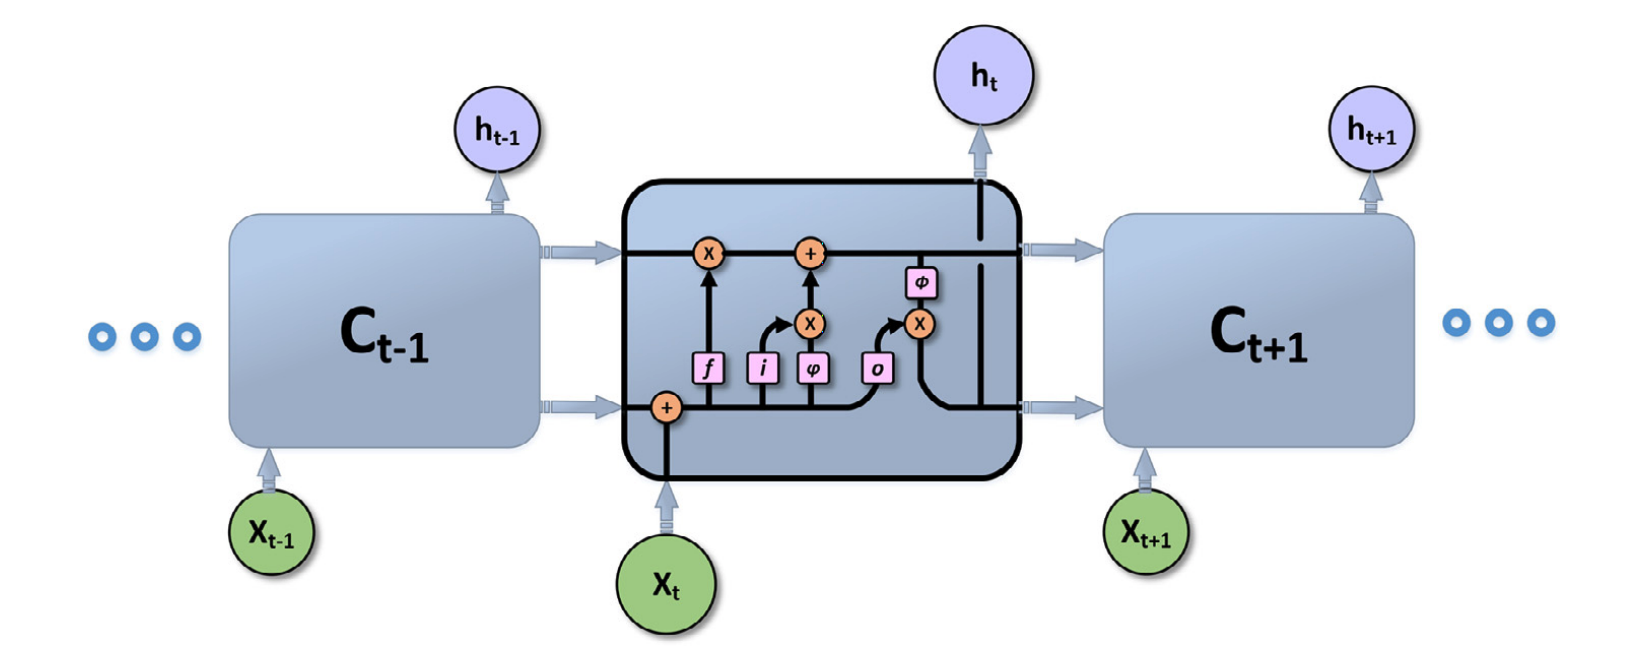
\includegraphics[scale=0.3]{LSTM.png}}
	\captionsetup{justification = centering}
	\caption{LSTM Cell Structure [5]}
	\label{fig:LSTM}
\end{figure*}

\subsection{LSTM Network Architecture}

The network architecture for a LSTM network utilizes a number of LSTM specific cells, shown in Figure 1,  to pass sequential data forward and ultimately provide a final prediction [5]. The two horizontal black lines show the flow of information; the bottom one is a signal composed of the current time and previous time input and the top one shows the state of the cell. Specifically, the bottom signal is used to update the value of the cell state and the nonlinear control signals. The top state splits into two directions: one signal to determine the cell output and the other fed into a new cell. Given the architecture, each LSTM cell, has the ability to remove or add information to the cell state through the nonlinear functions. Additionally, LSTM networks are known to reduce the "vanishing gradients" problem significantly during training; a common issue with RNN networks. 


\subsection{LSTM Neural Network Case Study}

In [6], a LSTM network was developed to classify a distracted driver based on driving behaviour through features such as velocity, acceleration, steering etc. The paper compared three data-driven networks: a memoryless MLP (Multilayer Perceptron) network, a stacked LSTM network and a stacked bi-directional LSTM network with an attention layer. In an effort to generate an effective database, the authors utilized a driving simulator and collected driving data on a group of volunteers. The topology of each network varied significantly in layering. First, the MLP network was designed to be a simple feed-forward network, set as a benchmark. Second, the stacked LSTM network utilized 2 layers of LSTM cells which passed data to a dense and output layer. The second LSTM network topology included 2 layers of LSTM cells as well as 2 layers of bidirectional LSTM cells which passed data to an attention, dense and output layer. The authors used the Rectilinear activation functions in the dense layer for both LSTM networks. Finally, the paper found that the attention layer reduces the total amount of training required to achieve the same accuracy relative to networks without an attention layer. As a result, the additional layer can be seen as a solution to reduce computation time. Additionally, the authors found that the attention layer enhances model accuracy from the results achieved; the layer significantly considers the weighted effect of the input data sequence on the output. 


A novel data-driven approach for estimating blood pressure using time domain features is proposed in [7]. Specifically, a LSTM network was used to learn the non-linear relationship between feature vector sequences and the target sequence. The paper utilizes distinct features such as cuff pressure, trough-to-peak amplitude, waveform slope etc. to feed into the network and ultimately determine a blood pressure estimate. For comparison, the paper tested other commonly used networks such as: Feed-Forward neural networks, Adaptive Neuro-Fuzzy Inference system, SVR (Support Vector Regression), Maximum Amplitude Algorithm (MAA) and Maximum/Minimum Slope Algorithm (MMSA). In particular, four different topologies of Feed-Forward networks were tested: 1 hidden layer with 9 neurons, 1 hidden layer with 10 neurons, 2 hidden layers with 11 neurons each, and 2 hidden layers with 9 neurons each. For these networks, the mean absolute error ranged from 8.9 to 9.2, where the stacked network of 11 neurons achieved the best results. Additionally, the ANFIS model achieved a mean absolute error (MAE) of 7.7 and the SVR model achieved a MAE of 9.8. The MAA and MSAA models also achieved a MAE of 15.2 and 9.1. In comparison, the LSTM-RNN model achieved significantly better results: MAE value of 3.8. Additionally, the authors show that using time-domain features of a wave signal can be used to effectively improve the accuracy of a LSTM network. 

For highly-variable time-series data, a wavelet transform LSTM model was developed in [8] and utilized to predict vehicle emissions: CO, HC and NO in advance. The emission database used in the paper was collected from a study done by the Urban Road Network Motor Vehicle Emission Monitoring System from May to December 2017. The system utilized a remote sensing equipment host, retroreflective sheeting and a license plate recognition system in order to measure the emission content. In terms of data preprocessing, the paper used the wavelet transform to decompose the highly variable time series data into several low-variable sub-series. Each subset was then fed into a LSTM network in order to predict the concentration of emissions. The sum of each series output was the determined overall emission concentration. For comparison purposes, the paper tests other networks such as: Autoregressive Integrated Moving Average (ARIMA) model, a standard LSTM network, and the combination wavelet-ARIMA and wavelet-LSTM. Based on the results, the paper found that the wavelet-LSTM network achieved a significantly lower MAE relative to the other networks. Additionally, the paper found that the addition of the wavelet transform does not improve performance when comparing wavelet-ARIMA to ARIMA and wavelet-LSTM to LSTM. The main benefit of the wavelet transform is that low-variable subseries data is more efficient computationally relative to using the original highly-variable time series data. 


\subsection{Neural Networks for RUL Applications}


Specific to RUL applications, one common deep learning approach in the research field is Recurrent Neural Networks (RNN). In [9], a RNN was designed to determine the health for a mechanical bearing experiencing degradation using the PRONOSTIA database and industrial experiments. First, the authors generate a subset using measurement data and time-frequency features from the PRONOSTIA database. Using this data, the authors then determine the features with the highest variance to use as the main inputs for the network. In total, the paper generated 11 bearing RUL datasets and used each one to train and test a RNN. For comparison, the paper tested a Self-Organizing Feature Map in an effort to benchmark the output. Based upon the results, the paper found that the SOM achieved an error of 53.24 and the RNN achieved a mean error of 32.48; significantly better than the SOM. 

Additionally, the authors tested the same networks with industrial data collected from wind turbines. Specifically, the authors installed accelerometers in order to monitor the health of a mechanical bearing. Similar to the first test, the authors compared the results of RNN and SOM networks. In particular, the SOM network achieved a mean error rate of 67.09 while the RNN achieved 23.24. Thus, the results clearly show that the RNN can achieve significantly better results for RUL applications in comparison to unsupervised data-driven approaches; namely SOM. 

Another popular neural network method for RUL applications is a Convolutional Neural Network (CNN). In [10], a multiscale CNN was used to estimate the remaining useful life of a bearing component. The architecture proposed was comprised of three stages of convolution and two stages of pooling layers, ending with a multi-scale and fully-connected layer. The paper utilizes a publicly available dataset: PRONOSTIA in the IEEE PHM 2012 Data Challenge. The dataset contains sensory data of a bearing experiencing a radial load force; resulting in bearing degradation. For data preprocessing, the paper used the wavelet transform to better utilize the frequency change in the dataset. For comparison, the paper tested other networks such as: MSCNN (Multiscale Convolutional Neural Network), RNN, SOM, and SVR (Support Vector Regression). Based upon the results, the paper found that the respective MAE was 1091.8, 1262, 1568, 1430. Additionally, the paper compared the result of the MSCNN to a standard CNN; where the CNN achieved a MAE of 1351. The authors found that due to the lower MAE achieved, the multiscale layer of the MSCNN proves to be advantageous in comparison with a standard CNN. Additionally, the MSCNN structure was found to keep global and local features throughout training such that the network can search for the best features of the entire dataset.  

In [11], a novel neural network topology was proposed to solve two main issues with CNNs for RUL applications. In particular, CNNs cannot be trained on temporal discrepancies of various degradation states thus, leading to potential increased error. Additionally, the predicted result of a CNN contains some degree of uncertainty which cannot be accurately determined. As a result, the authors propose a Recurrent Convolutional Neural Network (RCNN) approach for RUL estimation of machinery. First, recurrent convolutional layers are used to model temporal data of the various degradation states found within the dataset. Specifically, multiple recurrent convolutional and pooling layers are used which feed data into two fully-connected layers to produce the output. Once the prediction is determined, the authors utilized variation inference to determine the uncertainty of the result. For testing, the paper utilized vibrational data from the PRONOSTIA dataset as well as milling dataset found on NASA Prognostics Center of Excellence Data Repository. In terms of parameters, the paper found that the optimal parameters for the proposed network are the following: 4 layers, 100 neurons per layer, 128 batch size, 0.15 dropout probability and 200 epochs for training. The paper then compared the performance of the proposed network with the results of 4 other CNNs published in literature; varying in number of convolutional, pooling and fully-connected layers. Additionally, the paper used Cumulative Relative Accuracy (CRA) as a comparison metric between the networks. Based upon the results, the proposed network achieved a significantly higher CRA for the bearing dataset; maximum 0.8453. For the milling dataset, the proposed RCNN achieved a maximum CRA of 0.8601 while the highest CRA among the CNNs was 0.8171. Thus, the paper found that by stacking convolutional and pooling layers the network can better learn high-level representations and pass them into a fully-connected layer. As a result, a significantly better accuracy rate can be achieved in comparison to other published CNNs was shown. 



\subsection{LSTM Neural Networks for RUL Applications}


In [12], a novel LSTM network topology was used to determine the remaining useful life of a lithium-ion battery given features such as voltage, current and temperature charging profiles. In particular, the paper proposed a LSTM model using the "many-to-one" structure where multiple time-series input data are fed into the LSTM cell simultaneously; in an effort to reduce the number of total hyper-parameters. The dataset used in the paper is publicly available on the NASA Prognostics Center of Excellence Data Repository and features multiple battery datasets. Each dataset contains the charging, discharging and operating conditions of the battery over a period of time. In order to determine the best-suited hyper parameters, the authors iteratively test the error rate for various number of LSTM cells. The results show that 10 LSTM cells achieve the best results for all battery datasets however, the number of hidden nodes vary. Specifically, for battery 5, 6, 7 and 18, the number of hidden nodes used respectively is 9, 58, 13, and 4. Additionally, the authors found that the optimal learning rate and number of iterations were 0.001 and 500 through several iterations. For comparison, the paper test other neural networks such as: a standard LSTM, SC-LSTM, MC-RNN, MC-GRU, MC-SRU, MC-LSTM. Based upon the results, the MAPE achieved for each network are the following: 2.81, 1.71, 1.84, 1.51, 2.13 and 1.02. Thus, the LSTM model with the "many-to-one" structure clearly shows the best results. The authors found that the novel structure significantly reduces the number of parameters, improving variable generalization.  

In [13], an LSTM neural network was applied to the C-MAPSS dataset; revealing LSTM networks significantly outperform traditional neural networks in RUL applications. In particular, LSTM networks can learn and remember specific patterns within sensor data; providing an optimal method for detecting fault in degradation models. First, the authors utilized data preprocessing techniques to normalize the sensory data. The data was then fed into multiple neural networks and the results were compared. The paper compared the result from a stacked LSTM network with MLP, SVR, RVR and CNN models and found that LSTM networks can achieve a significantly lower error rate for RUL data. Specifically, the topology that achieved the best results was: a stacked LSTM network with 2 layers, each with 64 LSTM cells combined with 2 fully connected layers with 8 perceptron. This network was found to achieve a Root Mean Square Error (RMSE) of 4.596; the best result relative to other tested stacked LSTM networks. 

Additionally, the authors tested the various networks with two other datasets: PHM08 Challenge dataset and the Milling dataset found on the NASA repository. First, the PHM08 dataset was found to be similar to the C-MAPSS data however, the RUL values were not provided. In particular, the results of each tested network were uploaded to the NASA Data Repoistory Website were a single score was provided. For the following networks: MLP, SVR, RVR, CNN and Deep LSTM, the respective scores were found to be 3212, 15886, 8242, 3056 and 1862. Clearly, the Deep LSTM network was found to achieve the best results. Second, the same networks were tested with the Milling dataset. Similar to the other datasets, the Milling dataset provided sensory data for a milling machine as well as the remaining useful life estimate. The authors tested each network with this data and found the respective scores to be 6.26, 7.35, 17.22, 6.15 and 2.80; where the Deep LSTM network achieved significantly better results. Thus, the paper ultimately revealed that for RUL applications, a Deep LSTM network can be used to achieve a better error rate relative to other networks. 


For extremely complex RUL datasets, a hybrid LSTM network was developed better utilizing both long and short data sequences [14]. First, for long sequences, data smoothing techniques are used to preprocess the data and provide input into a LSTM network. Second, for short sequences, a predetermined time window is used to build a relation between RUL and present engine state. The combined data is passed to a feed-forward neural network to analyze the results and determine a prediction. For the CMAPPS dataset, the authors classified the each sensors data into three categories: ascending, descending and irregular. The irregular sensor dataset was found to not provide any useful information for the network thus, the authors removed that portion of the data for training and testing. For the parameters of the network, the authors found through iterative process that a LSTM layer of 10 cells, a learning rate of 0.006, and utilizing the ADAM optimizer provides the best results. The authors then compared the results of the network with other models including: a standard LSTM network, Time-Window Gradient Boosting Regression model, Time-Window Bayesian Ridge Regression model, Time-Window Support Vector Machine, and a Time-Window Linear Regression model; standard models used in the industry for RUL applications. The respective RMSE values determined for each model was found to be 0.158, 0.130, 0.157, 0.181, 0.159 and the hybrid model achieved 0.087. Thus, the paper found that a hybrid solution for long and short sequence time data can be an effective method for RUL applications in comparison to current industry models. 

\section{Problem Statement and the Dataset}
\label{Problem Statement and the Dataset}

The main goal of this paper is, then, to design and develop a LSTM-based network in order to accurately predict the RUL for a turbofan engine, given its historical failure data. To achieve this, several LSTM networks topologies shall be designed varying in topologies, evaluated on the testing database and analyzed. As a result, a deep learning approach for RUL estimation can, then, be potentially used within the PHM system in order to effectively schedule maintenance; minimizing maintenance labour cost and operational downtime. 

The main dataset used in this paper is the turbofan engine degradation dataset publicly available on the NASA Prognostics and Center of Excellence Data Repository. In particular, the dataset includes four simulated turbofan systems during different operating conditions. Each dataset is then split into training and testing subsets; the training subset contains the target remaining useful life vector whereas the testing subset does not. At the beginning of the training subset, the engine operates normally until a random fault occurs, which builds in magnitude until there is system failure. Within the dataset, there are 26 columns: The first column indicates engine ID, second column indicates current operational cycle, 3-5 represent engine operational settings and 6-26 show the sensory data of the engine. In the testing dataset, data is provided an unknown time prior to system failure. The goal is then to predict the number of remaining useful lifecycles of the turbofan engine. 


\begin{thebibliography}{10}

\bibitem{Chiesa} S. Chiesa, S. Quer, S. Corpino and N. Viola, "Heuristic and exact techniques for aircraft maintenance scheduling," \emph{Proceedings of the Institution of Mechanical Engineers, Part G: Journal of Aerospace Engineering,} vol. 223, no. 7, pp. 989-999, 2009. 

\bibitem{Baybutt} M. Baybutt, C. Minnella, A. E. Ginart, P. W. Kalgren and M. J. Roemer, "Improving Digital System Diagnostics Through Prognostic and Health Management (PHM) Technology," \emph{IEEE Transactions on Instrumentation and Measurement,} vol. 58, no. 2, pp. 255-262, 2009. 

\bibitem{Zhou}X. Si, W. Wang, C. Hu and D. Zhou, "Remaining useful life estimation - A review on the statiscal data driven approaches," \emph{European Journal of operational Research,} vol. 213, no. 1, pp. 1-14, 2011. 


\bibitem{Zerhouni} A. Mosallam, K. Medjaher and N. Zerhouni, "Data-driven prognostic method based on Bayesian approaches for direct remaining useful life prediction," \emph{Journal of Intelligent Manufacturing,} vol. 27, no. 5, pp. 1037-1048, 2016. 

\bibitem{Liu} Y. Wu, M. Yuan, S. Dong, L. Lin and Y. Liu, "Remaining useful life estimation of engineered system using vanilla LSTM neural networks," \emph{Neurocomputing,} vol. 275, pp. 167-179, 2018. 

\bibitem{Gaffar}S. M. Kouchak and A. Gaffar, "Detecting Driver Behaviour Using Stacked Long-Short Term Memory Network with Attention Layer," \emph{IEEE Transactions on Intelligent Transportation Systems,} pp. 1-10, 2020. 

\bibitem{Celler}A. Argha and B. G. Celler, "Blood Pressure Estimation From Time-Domain Features of Oscillometric Waveforms using Long Short-Term Memory Recurrent Neural Networks," \emph{IEEE Transactions on Instrumentation and Measurement,} vol. 69, no. 6, pp. 3614-3622, 2020. 

\bibitem{Ling}Q. Zhang, F. Li, F. Long and Q. Ling, "Vehicle Emission Forecasting Based on Wavelet Transform and Long Short-Term Memory Network," \emph{IEEE Access, }vol. 6, pp. 56984-56994, 2018. 

\bibitem{Liang}G. Liang, N. Li, F. Jia, Y. Lei and J. Lin, "A recurrent neural network based on health indicator for remaining useful life prediction of bearings," \emph{Neurocomputing,} vol. 379, pp. 117-129, 2020. 
\bibitem{Peng}J. Zhu, N. Chen and W. Peng, "Estimation of Bearing Remaining Useful Life Based on Multiscale Convolutional Neural Network," \emph{IEEE Transactions on Industrial Electronics, }vol. 66, no. 4, pp. 3208-3216, 2019. 
\bibitem{Guo}B. Wang, Y. Lei, T. Yan, N. Li and L. Guo, "Recurrent convolutional neural network: A new framework for remaining useful life prediction of machinery," \emph{Neurocomputing, }vol. 379, pp. 117-129, 2020. 
\bibitem{Kim}K. Park, Y. Choi, W. J. Choi, H. Ryu and H. Kim, "LSTM-Based Battery Remaining Useful Life With Multi-Channel Charging Profiles," \emph{IEEE Access, }vol. 8, pp. 20786-20798, 2020. 
\bibitem{Gupta}S. Zheng, K. Ristovski, A. Farahat and C. Gupta, "Long Short-Term Memory Network for Remaining Useful Life Estimation," \emph{2017 IEEE International Conference on Prognostics and Health Management (ICPHM), }pp. 88-95, 2017. 
\bibitem{Huang}S. Wang, X. Zhang, D. Gao, B. Chen, Y. Cheng, Y. Yang, W. Yu, Z. Huang and J. Peng, "A Remaining use Life Prediction Model Based on Hybird Long-Short Sequences for Engines," \emph{2018 21st International Conference on Intelligent Transportation Systems (ITSC), }  pp. 1757-1762, 2018. 


\end{thebibliography}





\end{document}

